%%==================================================
%% chapter02.tex for TJU Master Thesis
%% based on CASthesis
%% modified by wei.jianwen@gmail.com
%% Encoding: UTF-8
%%==================================================

\chapter{衰减介质理论基础}

线性粘弹理论已趋于完善,\citeB{carcione:2007} 对其做了较为完整的总结。粘弹性介质的性质介于弹性固体与粘性流体之间,
可以定义为材料在一定的外力作用历史条件及其处于某一温度范围情况下所表现出来的同时具有弹性固体和粘性流体效应的性质。
除了当时所受外力大小外,外力加载时间、加载历史以及介质温度变化都会对粘性介质的形变产生影响。粘弹性介质的行为是介质
的应变率决定的,它随时间的变化逐渐表现出来。外力的加载过程和介质的形变历史决定了介质的应力-应变关系,这也就是说介质
是具有记忆性的,而弹性介质的应力-应变关系是瞬时线性的。本章简要回顾衰减理论及其表征,总结常用的描述衰减机制的
物理模型,并系统总结在地震学中常用的几类描述衰减性的粘声波动方程。

\vspace{1.0cm}

\section{衰减理论及其表征}

假定介质的性质不随时间变化,在等温条件下本构方程描述的应力-应变关系是一种褶积关系。用等效力学模型可以描述一般化的非弹性
现象,这种模型一般用弹簧和阻尼器线性组合而成。能量储存在弹簧中而耗散在阻尼器中,弹簧和阻尼器任意串联/并联即可以提供一个
很好的现象学模型来研究聚合物、岩石等材料的粘弹性质。


\vspace{0.5cm}

\subsection{复模量及耗散存储模量}

在弹性介质中,Hooke 定律表示为:
\begin{equation}
	\sigma = M_e\epsilon,
	\label{eq:stress_strain}
\end{equation}
其中$\sigma,\epsilon,M_e$分别表示应力、应变和弹性模量。而根据定义,粘弹介质中本构关系表示为:
\begin{equation}
	\sigma = \varphi*\partial_t\epsilon,
	\label{eq:visco_hooke}
\end{equation}
其中$\varphi$为驰豫函数,$*$表示褶积运算。对方程~\ref{eq:visco_hooke}做Fourier变换有:
\begin{equation}
	F[\sigma(\omega)]=M(\omega)F[\epsilon(\omega)],
	\label{eq:vis_stress_strain}
\end{equation}
其中$F[\cdot]$为Fourier变换算子,并且
\newpage
\begin{equation}
	M(\omega)=F[\partial_t\varphi(\omega)]=\int_{-\infty}^{\infty}\partial_t\varphi(t)\exp(-i\omega t)dt,
	\label{eq:fourier}
\end{equation}
为复模量。把复模量分解为实部和虚部$M(\omega)=M_1(\omega)+M_2(\omega)$,其中$M_1(\omega)$为存储模量,
$M_2(\omega)$为耗散模量,且有:
\begin{equation}
	\left\lbrace
	\begin{aligned}
		M_1(\omega) &=\omega\int_{0}^{\infty}sin(\omega t)dt \\ 
		M_2(\omega) &=\omega\int_{0}^{\infty}[\varphi(t)-\varphi(\infty)]cos(\omega t)dt.
	\end{aligned} \right
\end{equation} 
定义应变-应力关系为
\begin{equation}
	\epsilon=\chi*\partial_t\sigma,
\end{equation}
其中$\chi$为蠕变函数,由$\sigma=\partial_t\varphi*\epsilon=\partial_t\varphi*(\partial_t\chi*\sigma)
=(\partial_t\varphi*\partial_t\chi)*\sigma$有$\partial_t\varphi(t)*\partial_t\chi(t)=\delta(t)$,即:
$M(\omega)J(\omega)=1$,其中$J(\omega)=F[\partial_t\chi]$。

\vspace{0.8cm}
\subsection{品质因子与衰减系数}
\vspace{0.2cm}
频率域的应力-应变关系(\ref{eq:vis_stress_strain})跟弹性介质在时间域的应力-应变关系(\ref{eq:stress_strain})
有相同的表达式,但是模量是复数并且与频率有关。用波动方程一维平面波解可以清晰显示这种关系,其解的形式为:
\begin{equation}
	u=u_0\exp[i(\omega t-kx)],
	\label{eq:plane_wave}
\end{equation}
其中$k$为波数,$\omega$为频率,介质内部与表面力平衡满足如下关系:
\begin{equation}
	\partial_x\sigma=\rho\partial^2_{tt}u,
\end{equation}
假定介质的性质恒定,由$\epsilon=\partial_t u$及公式(\ref{eq:vis_stress_strain})可以得出方程(\ref{eq:plane_wave})
的频散关系
\begin{equation}
	M(\omega)k^2=\rho\omega^2.
\end{equation}
对于波在粘性介质中传播来说,$k$是复数,$\omega$是实数,可以得出波传播的复速度:
\begin{equation}
	v_c(\omega)=\frac{\omega}{k}=\sqrt{\frac{M(\omega)}{\rho}}
	\label{eq:vc}
\end{equation}
把复波数表示为:
\begin{equation}
	k=\kappa -i\alpha,
\end{equation}
\newpage
方程(\ref{eq:plane_wave})可以重新表示为:
\begin{equation}
	u=u_0\exp(-\alpha x)\exp[i(\omega t-\kappa x)],
\end{equation}
其中$\kappa$为波数,$\alpha$为衰减系数。定义相速度为:
\begin{equation}
	v_p=\frac{\omega}{\kappa}=[Re(\frac{1}{v_c})]^{-1}
	\label{eq:phase_velocity}
\end{equation}
衰减系数为:
\begin{equation}
	\alpha=-\omega Im(\frac{1}{v_c}),
	\label{eq:alpha}
\end{equation}
其中$Re(\cdot)$,$Im(\cdot)$分别为取实部和虚部运算。
在弹性介质中频率对波数的导数即为群速度,在粘弹介质中,只考虑实波数$\kappa$:
\begin{equation}
	v_g=\frac{\partial \omega}{\partial \kappa}=(\frac{\partial \kappa}{\partial \omega})^{-1}
	=[Re(\frac{\partial k}{\partial \omega})]^{-1}.
\end{equation}
能量的耗散也可以用品质因子$Q$来定量表征,$Q^{-1}$叫做耗散因子。品质因子可表示为模量的实部与模量的
虚部的比值,
\begin{equation}
	Q=\frac{M_1}{M_2}=\frac{Re(v_c^2)}{Im(v_c^2)}=-\frac{Re(k^2)}{Im(k^2)}.
	\label{eq:qm}
\end{equation}
因为$k^2=\kappa^2-\alpha^2-2i\kappa\alpha$,品质因子跟衰减系数和波数之间的关系可表述为:
\begin{equation}
	\alpha=(\sqrt{Q^2+1}-Q)\kappa,
	\label{eq:q_alpha}
\end{equation}
在低衰减介质中,$Q>>1$,把(\ref{eq:phase_velocity})式跟$f=\omega/(2\pi)$带入(\ref{eq:q_alpha})
中,并用Taylor级数展开有:
\begin{equation}
	\alpha=\frac{\kappa}{2Q}=\frac{\omega}{2Qv_p}=\frac{\pi f}{Qv_p}.
	\label{eq:linear_visco}
\end{equation}
衰减系数$\alpha$与频率$f$呈线性关系,即所谓的线性衰减。

\section{描述衰减性的基本模型}
\vspace{0.2cm}
弹簧和阻尼器简单的串/并联可以组合成描述衰减的不同力学模型。Maxwell 在1967年提出了用来描述气体粘滞性问题的Maxwell模型;
Meyer和Voigt通过经典的弹性波方程总结出了所谓的Voigt应力-应变关系,由Kelvin在1875年提出了代表Voigt固体的力学模型--
Kelvin-Voigt模型;Poynting和Thomson在1902年提出更能代表真实介质材料的Zener模型或标准线性固体模型。在油气勘探
和地震学中,由于不知道衰减与频率的依赖关系,经常用多个Zener模型并联在一起来表示近似常$Q$模型,并用气刻画岩石
的衰减特性。在勘探地震频段,\citeB{kjartansson:1979}提出了理想的常$Q$线性衰减模型。

模型的驰豫函数可以通过对模型瞬间施加一个恒定的单位应变$\epsilon=H(t)$,然后测量其应力的变化,即
\begin{equation}
	\sigma(t)=\partial_t\varphi(t)*H(t)=\varphi(t)*\delta(t)=\varphi(t).
\end{equation}
对模型瞬间施加一个恒定的单位应力$\delta=H(t)$,测定其应变随时间的变化即可得到模型的蠕变函数,
\begin{equation}
	\epsilon(t)=\partial_t\chi(t)*H(t)=\chi(t)*\delta(t)=\chi(t).
\end{equation}
在恒力的情况下,应变不随时间变化而变化的是弹性固体,应变以等应变率随时间增加的是粘性流体。
图\ref{fig:strain}反应了在恒定应力作用下应变蠕变曲线,图\ref{fig:stress}反应了在恒定应变下的应力松弛曲线。
\begin{figure*}[!htbp]
	    \centering
		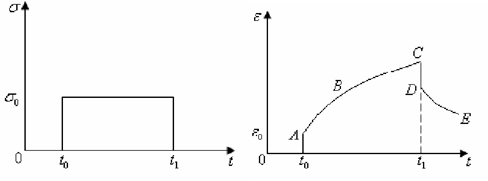
\includegraphics[width=0.9\linewidth]{figure/strain}
	    \fcaption{弹性和粘弹性固体的应变蠕变回复曲线}{Creep function of elasticity and 
					visco-elasticity}[介质应变蠕变回复曲线]
		\label{fig:strain}
\end{figure*}
\begin{figure*}[!htbp]
	    \centering
		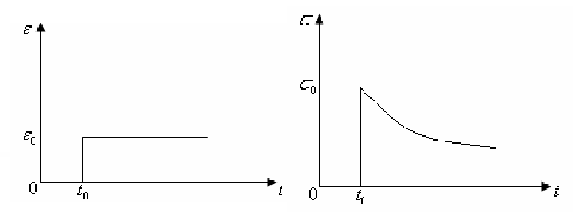
\includegraphics[width=0.95\linewidth]{figure/stress}
	    \fcaption{弹性和粘弹性固体的应力松驰曲线}{Relaxation function of elasticity and 
					visco-elasticity}[介质应力松驰曲线]
		\label{fig:stress}
\end{figure*}


\vspace{0.2cm}
\subsection{Maxwell模型}
\vspace{0.2cm}
如图\ref{fig:maxwell_model}所示,弹簧与阻尼器简单的串联即可得到Maxwell模型。对模型施加一个
应力$\sigma$,就会在模型的弹簧中产生形变$\epsilon_1$,并在阻尼器中产生形变$\epsilon_2$。
弹簧中的应力-应变关系为:
\begin{equation}
	\sigma=M_U\epsilon_1,
\end{equation}
其中$M_u$是弹簧的弹性模量,下标$U$表示“无驰豫”。阻尼器中的应力-应变关系为:
\begin{equation}
	\sigma=\eta\partial_t \epsilon_2, \quad \eta\geq0,
\end{equation}
其中$\eta$为粘滞系数。
\begin{figure*}[!htbp]
	    \centering
		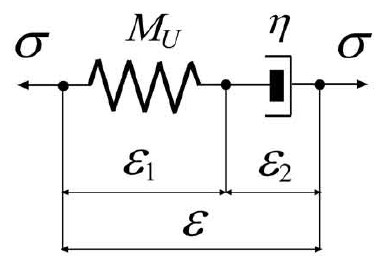
\includegraphics[width=0.6\linewidth]{figure/maxwell_model}
	    \fcaption{Maxwell模型}{Maxwell model}[Maxwell模型]
		\label{fig:maxwell_model}
\end{figure*}
假设系统的总形变量为$\epsilon=\epsilon_1+\epsilon_2$,则Maxwell模型对应的应力-应变关系为:
\begin{equation}
	\frac{\partial_t\sigma}{M_U}+\frac{\sigma}{\eta}=\partial_t\epsilon.
	\label{eq:stress_maxwell}
\end{equation}
对方程(\ref{eq:stress_maxwell})两边做Fourier变换有
\begin{equation}
	\sigma=M\epsilon,
\end{equation}
其中$M(\omega)=\frac{\omega\eta}{\omega\tau-i}$是复模量,并且满足驰豫时间
$\tau=\frac{\eta}{M_U}$。由(\ref{eq:fourier})式可得其相应的驰豫函数为:
\begin{equation}
	\varphi(t)=M_U\exp(-t/\tau)H(t).
\end{equation}
由$M(\omega)J(\omega)=1$可以推到出$Maxwell$模型的蠕变函数,
\begin{equation}
	\chi(t)=\frac{1}{M_U}(1+\frac{t}{\tau})H(t).
\end{equation}
Maxwell模型($M_U=2.16GP_a,\tau=1/(2\pi f),f=25Hz$)的蠕变和驰豫函数如图\ref{fig:maxwell_creep}
所示,蠕变函数并不能代表真实固体中的蠕变行为,而是类似于粘性流体的蠕变函数。
\begin{figure*}[!htbp]
	    \centering
		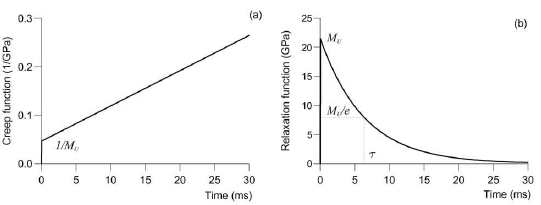
\includegraphics[width=0.9\linewidth]{figure/maxwell_creep}
		\fcaption{Maxwell模型的蠕变(a)和驰豫(b)函数}{The creep and relaxation function 
		of Maxwell model}[Maxwell模型的蠕变和驰豫函数]
		\label{fig:maxwell_creep}
\end{figure*}
在松弛实验中,弹簧和阻尼器受同样大小的力,由于阻尼器不能产生瞬间的形变,因此最初的伸展出现在
弹簧中。阻尼器扩张而弹簧压缩,所以导致模型的总拉伸量相等。最后弹簧中的应力全部释放,而驰豫函数
不像真实固体中的那样呈现双曲关系的剩余应力,所以Maxwell模型适合代表粘滞性流体模型。从图
\ref{fig:maxwell_creep}(a)中可以看出$M_U$代表系统的瞬时响应,所以叫做无驰豫的模量。
地震波的传播属性被介质的相速度、衰减系数以及品质因子所描述。Maxwell模型的品质因子有如下
简单的表达形式:
\begin{equation}
	Q(\omega)=\frac{Re(M)}{Im(M)}=\omega\tau.
\end{equation}
模型($M_U=\rho c^2, \rho=2.4g/cm^3, c=3km/s, \tau=1/(2\pi f), f=25Hz$)的相速度和耗散因子如
图\ref{fig:maxwell_vp}所示。当$\omega\to0$时,$v_p=0$,当$\omega\to\infty$时,$v_p\to\sqrt{M_U/\rho}$
即处于弹性状态。这表明波在Maxwell模型中的传播速度慢于在用弹簧代表的弹性固体中的传播速度。耗散因子
在零频率成分时为无穷大,在高频时表现为无衰减特性。
\begin{figure*}[!htbp]
	    \centering
		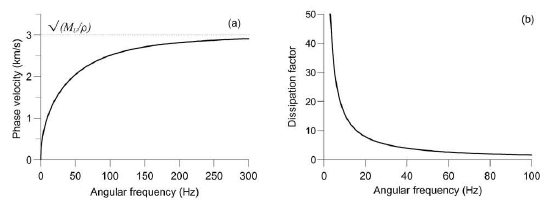
\includegraphics[width=0.8\linewidth]{figure/maxwell_vp}
		\fcaption{Maxwell模型的相速度(a)和耗散因子(b)}{The phase velocity and dissipation factor 
		of Maxwell model}[Maxwell模型的相速度和耗散因子]
		\label{fig:maxwell_vp}
\end{figure*}


\vspace{0.5cm}
\subsection{Kelvin-Voigt模型}
\vspace{0.5cm}
在弹性力学中,通常用Kelvin-Voigt应力-应变关系来描述粘弹介质模型,其模型由弹簧和阻尼器并联而成
(图\ref{fig:kelvin_model})
\begin{figure*}[!htbp]
	    \centering
		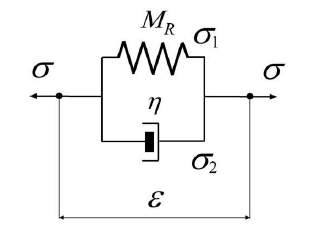
\includegraphics[width=0.6\linewidth]{figure/kelvin_model}
	    \fcaption{Kelvin-Voigt模型}{Kelvin-Voigt model}[Kelvin-Voigt模型]
		\label{fig:kelvin_model}
\end{figure*}
总的应力可以分解成弹性应力与粘性应力:
\begin{equation}
	\left\lbrace
	\begin{aligned}
		\sigma_1=M_R\epsilon, \\
		\sigma_2=\eta\partial_t\epsilon,
	\end{aligned} \right
\end{equation}
其中$M_R$为弹簧模量,下标$R$表示“驰豫”,$\epsilon$为系统的总应变。其应力-应变关系为
\begin{equation}
	\sigma=\sigma_1+\sigma_2=M_R\epsilon+\eta\partial_t\epsilon.
	\label{eq:kelvin}
\end{equation}
对(\ref{eq:kelvin})式做Fourier变换有:
\begin{equation}
	\sigma=(M_R+i\omega\eta)\epsilon,
\end{equation}
即可得出复模量为$M(\omega)=M_R+i\omega\eta$。
Kelvin-Voigt模型的驰豫函数为:
\begin{equation}
	\varphi(t)=M_RH(t)+\eta\delta(t),
\end{equation}
其蠕变函数为:
\begin{equation}
	\chi(t)=\frac{1}{M_R}[1-\exp(-t/\tau)]H(t),
\end{equation}
其中$\tau=\eta/M_R$。

Kelvin-Voigt模型($M_R=2.16GP_a,\tau=1/(2\pi f),f=25Hz$)的驰豫函数和蠕变函数如图\ref{fig:kelvin_creep}
所示。驰豫函数与时间无关,这是一种纯弹性固体。$\delta$函数表明在实际中对介质施加一个瞬时应变是不可能的。
阻尼器最先开始拉伸然后转换成应力存储于弹簧中。最后,剩余应力都存储于弹簧中。阻尼器不能瞬间移动导致蠕变
函数不能表示瞬时应变。这不是真实的固体介质,蠕变函数当时间趋于无穷时趋近于驰豫模量$M_R$。
\begin{figure*}[!htbp]
	    \centering
		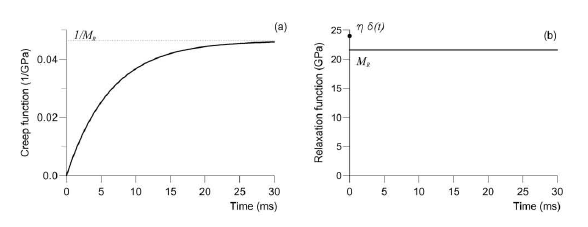
\includegraphics[width=0.9\linewidth]{figure/kelvin_creep}
		\fcaption{Kelvin-Voigt模型的蠕变(a)和驰豫(b)函数}{The creep and relaxation function 
		of Kelvin-Voigt model}[Kelvin-Voigt模型的蠕变和驰豫函数]
		\label{fig:kelvin_creep}
\end{figure*}
\begin{figure*}[!htbp]
	    \centering
		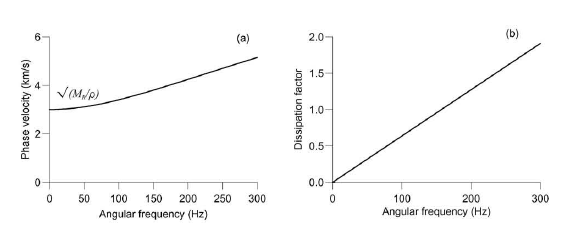
\includegraphics[width=0.8\linewidth]{figure/kelvin_vp}
		\fcaption{Kelvin-Voigt模型的相速度(a)和耗散因子(b)}{The phase velocity and dissipation factor 
		of Kelvin-Voigt model}[Kelvin-Voigt模型的相速度和耗散因子]
		\label{fig:kelvin_vp}
\end{figure*}
Kelvin-Voigt模型的品质因子为:
\begin{equation}
	Q(\omega)=(\omega\tau)^{-1}.
\end{equation}
Kelvin-Voigt模型的品质因子与Maxwell模型的品质因子互为倒数。Kelvin-Voigt模型($M_R=\rho c^2,
\rho=2.4g/cm^3,c=3km/s,\tau=1/(2\pi f),f=25Hz $)的相速度和耗散因子如图\ref{fig:kelvin_vp}所示。
当$\omega\to0$时,$v_p\to\sqrt{M_R/\rho}$;当$\omega\to\infty$时,$v_p\to\infty$。这表明波
在Kelvin-Voigt模型中的传播速度比在相应的弹性介质中的速度大。


\vspace{0.2cm}
\subsection{Zener模型或标准线性固体模型}
\vspace{0.2cm}
Zener或标准线性固体模型由弹簧跟Kelvin-Voigt模型串联形成(图\ref{fig:sls_model})。该模型更能代表真实介质,如
岩石、聚合物以及金属材料。
\begin{figure*}[!htbp]
	    \centering
		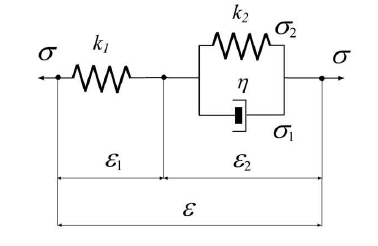
\includegraphics[width=0.6\linewidth]{figure/sls_model}
	    \fcaption{标准线性固体模型}{Standard linear solid model}[标准线性固体模型]
		\label{fig:sls_model}
\end{figure*}
标准线性固体模型的应力-应变关系为:
\begin{equation}
	\left\lbrace
	\begin{aligned}
		\sigma&=\kappa_1\epsilon_1, \\
		\sigma_1&=\eta\partial_t\epsilon_2, \\
		\sigma_2&=\kappa_2\epsilon_2, 
	\end{aligned} \right
\end{equation}
其中$\kappa_1\geq0,\kappa_2\geq0,\eta\geq0$,并且
\begin{equation}
	\sigma=\sigma_1+\sigma_2, \quad \epsilon=\epsilon_1+\epsilon_2.
\end{equation}
上述方程的解给出了标准线性固体模型的应力-应变关系:
\begin{equation}
	\sigma+\tau_\sigma\partial_t\sigma=M_R(\epsilon+\tau_\epsilon\partial_t\epsilon),
\end{equation}
其中$M_R=\frac{\kappa_1\kappa_2}{\kappa_1+\kappa_2}$为拉伸模量,驰豫时间满足$\tau_\sigma=
\frac{\eta}{\kappa_1+\kappa_2}\tau_\epsilon=\frac{\eta}{\kappa_2}\geq\tau_\sigma$。
其中复模量为:
\begin{equation}
	M(\omega)=M_R\frac{1+i\omega\tau_\epsilon}{1+i\omega\tau_\sigma}
\end{equation}
驰豫模量$M_R$由$\omega=0$时得到,未驰豫模量$M_U$由$\omega\to\infty$时得到,且为$M_U=M_R
\frac{\tau_\epsilon}{\tau_\sigma}$。
标准线性固体模型的驰豫函数为:
\begin{equation}
	\varphi(t)=M_R[1-(1-\frac{\tau_\epsilon}{\tau_\sigma})\exp(-t/\tau_\sigma)]H(t),
\end{equation}
其蠕变函数为:
\begin{equation}
	\chi(t)=\frac{1}{M_R}[1-(1-\frac{\tau_\epsilon}{\tau_\sigma})\exp(-t/\tau_\epsilon)]H(t).
\end{equation}
标准线性固体模型($M_R=2.16GP_a,M_U=29.4GP_a,\tau_0=1/(2\pi f),f=25Hz$)的驰豫函数和蠕变函数
如图\ref{fig:sls_creep}所示。
\begin{figure*}[!htbp]
	    \centering
		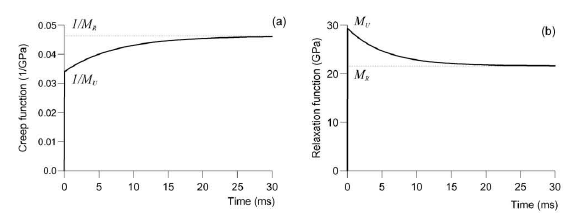
\includegraphics[width=0.9\linewidth]{figure/sls_creep}
		\fcaption{标准线性固体模型的蠕变(a)和驰豫(b)函数}{The creep and relaxation function 
		of standard linear solid model}[标准线性柜台模型的蠕变和驰豫函数]
		\label{fig:sls_creep}
\end{figure*}
\begin{figure*}[!htbp]
	    \centering
		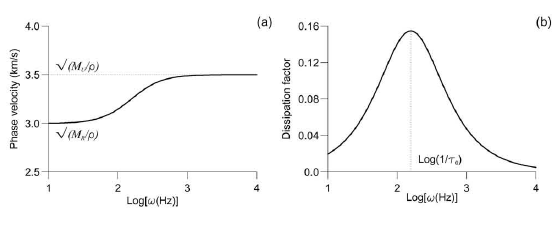
\includegraphics[width=0.8\linewidth]{figure/sls_vp}
		\fcaption{标准线性固体模型的相速度(a)和耗散因子(b)}{The phase velocity and dissipation factor 
		of standard linear solid model}[标准线性固体模型的相速度和耗散因子]
		\label{fig:sls_vp}
\end{figure*}
在蠕变实验中,蠕变由一个由弹簧常数决定的瞬间初始值$\chi(0^+)=M_U^{-1}$逐渐达到其渐进逼近值
$\chi(\infty)=M_R^{-1}$。经过一个初始位移后,应力由于阻尼器变形的增加而逐渐降低,最终使应变达到逼近值。
类似地,驰豫函数经过短暂的处于拉伸状态的$M_U$后,最终达到拉伸模量$M_R$。
标准线性固体模型的品质因子为:
\begin{equation}
	Q(\omega)=\frac{1+\omega^2\tau_\epsilon\tau_\sigma}{\omega(\tau_\epsilon-\tau_\sigma)}.
\end{equation}
标准线性固体模型($M_R=\rho c_R^2,\rho=2.4g/cm^3,c_R=3km/s,M_U=\rho c_U^2,c_U=3.5km/s,f=25Hz$)的
相速度和耗散因子$Q^{-1}$如图\ref{fig:sls_vp}所示。
模型在$\omega_0=1/\tau_0$处有拉伸峰值,其中$\tau_0=\sqrt{\tau_\epsilon\tau_\sigma}$。相速度随着频率的增加
而增加,且在低频时的$\sqrt{M_R/\rho}$与高频时的$\sqrt{M_U/\rho}$之间变化,当介质为纯弹性体($Q^{-1}=0$)
时,$M_R=M_U$。



\vspace{0.9cm}
\subsection{广义Zener模型/近似常$Q$模型}
\vspace{0.1cm}
在油气勘探和地震学中,由于不知道衰减与频率的依赖关系,用常$Q$模型刻画岩石的吸收衰减会更方便。物理实验表明
衰减系数在许多频率范围内与频率呈线性关系,即品质因子为常数。通常用多($L$)个Zener模型单元并联在一起组成广义
Zener模型来近似常$Q$模型(图\ref{fig:zener})。
\begin{figure*}[!htbp]
	    \centering
		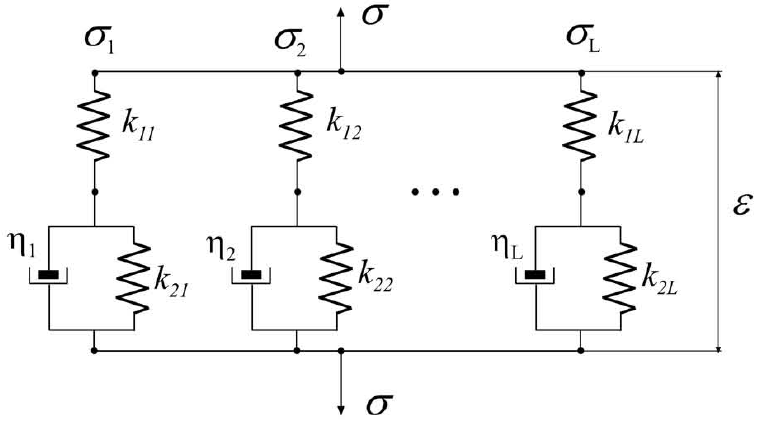
\includegraphics[width=0.7\linewidth]{figure/zener}
	    \fcaption{广义Zener模型}{Generalized Zener model}[广义Zener模型]
		\label{fig:zener}
\end{figure*}
每个小Zener模型单元的应力-应变关系为:
\begin{equation}
	\sigma_l+\tau_{\sigma l}\partial_t\sigma_l=M_{Rl}(\epsilon+\tau_{\epsilon l}
	\partial_t\epsilon), \quad l=1,\cdots L,
\end{equation}
其中驰豫模量为:
\begin{equation}
	M_{Rl}=\frac{\kappa_{1l}\kappa_{2l}}{\kappa_{1l}+\kappa_{2l}}
\end{equation}
驰豫时间为:
\begin{equation}
	\tau_{\sigma l}=\frac{\eta_l}{\kappa_{1l}+\kappa_{2l}} \quad \tau_{\epsilon l}=
	\frac{\eta_l}{\kappa_{2l}}.
\end{equation}
每个小单元的复模量:
\begin{equation}
	M_l(\omega)=M_{Rl}\frac{1+i\omega\tau_{\epsilon l}}{1+i\omega\tau_{\sigma l}}
\end{equation}
弹性系统的总应力为$\sigma=\sum_{l=1}^{L}\sigma_l$,频率域的应力-应变关系为
\begin{equation}
	\sigma=\sum_{l=1}^{L}M_l\epsilon=\sum_{l=1}^{L}M_{Rl}\frac{1+i\omega\tau_{\epsilon l}}
	{1+i\omega\tau_{\sigma l}}\epsilon.
\end{equation}
选择$M_{Rl}=M_R/L$,复模量可以表示成:
\begin{equation}
	M(\omega)=\sum_{l=1}^{L}M_l(\omega), \quad M_l(\omega)=\frac{M_R}{L}
	(\frac{1+i\omega\tau_{\epsilon l}}{1+i\omega\tau_{\sigma l}})
\end{equation}
由此可以把独立常数减少至$2L+1$个。驰豫函数很容易由时间域的本构关系得到,
\begin{equation}
	\varphi(t)=M_R[1-\frac{1}{L}\sum_{l=1}^{L}(1-\frac{\tau_{\epsilon l}}{\tau_{\sigma l}})
	\exp(-t/\tau_{\sigma l})]H(t),
\end{equation}
当$t=0$时,未驰豫模量为:
\begin{equation}
	M_U=M_R[1-\frac{1}{L}\sum_{l=1}^{L}(1-\frac{\tau_{\epsilon l}}{\tau_{\sigma l}})]
	=\frac{M_R}{L}\sum_{l=1}^{L}\frac{\tau_{\epsilon l}}{\tau_{\sigma l}}.
\end{equation}
单Zener元件的品质因子可以通过中心频率$\omega_0=\tau_0^{-1}$处的品质因子
\begin{equation}
	Q_0=\frac{2\tau_0}{\tau_\epsilon-\tau_\sigma}
	\label{eq:qq}
\end{equation}
表示:
\begin{equation}
	Q(\omega)=Q_0\frac{1+\omega^2\tau_0^2}{2\omega\tau_0}.
\end{equation}
将$\tau_0=\sqrt{\tau_\epsilon\tau_\sigma}$代入方程\ref{eq:qq}中有
\begin{equation}
	\tau_\epsilon=\frac{\tau_0}{Q_0}(\sqrt{Q_0^2+1}+1), \quad \tau_\sigma=\frac{\tau_0}{Q_0}(\sqrt{Q_0^2+1}-1).
\end{equation}
寻找一系列驰豫时间$\tau_{\epsilon l}$和$\tau_{\sigma l}$,使得在给定的中心频率$\omega_{0l}=1/\tau_{0l}$附近品质因子
$Q$呈常数。单驰豫的峰值应均匀分布在$log(\omega)$尺度内,整个系统的品质因子为:
\begin{equation}
	Q(\omega)=\frac{Re(M)}{Im(M)}=\frac{Re(\sum_{l=1}^{L}M_l)}{Im(\sum_{l=1}^{L}M_l)}.
\end{equation}
\begin{figure*}[!htbp]
	    \centering
		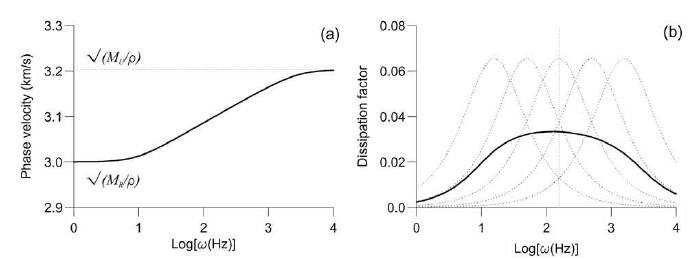
\includegraphics[width=0.8\linewidth]{figure/zener_vp}
		\fcaption{广义Zener模型的相速度(a)和耗散因子(b)}{The phase velocity and dissipation factor 
		of generalied Zener model}[广义Zener模型的相速度和耗散因子]
		\label{fig:zener_vp}
\end{figure*}
\begin{figure*}[!htbp]
	    \centering
		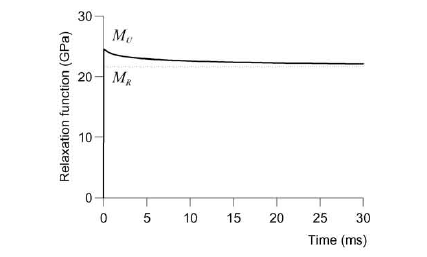
\includegraphics[width=0.7\linewidth]{figure/zener_rela}
		\fcaption{广义Zener模型的驰豫函数}{The relaxation function 
		of standard linear solid model}[广义Zener模型的驰豫函数]
		\label{fig:zener_rela}
\end{figure*}
图\ref{fig:zener_vp}显示了5个Zener单元的相速度和衰减系数随频率的变化关系,其品质因子为30,其中每个单元的
品质因子参数为$Q_0=15$。点划线表示每个单元的品质因子,竖直点划线为第三个单元的驰豫峰值。该近似常$Q$模型的
驰豫函数如图\ref{fig:zener_rela}所示。


\vspace{0.5cm}
\subsection{常$Q$模型}
\vspace{0.5cm}
对所有的频率段,都可以设计出非常理想的常$Q$模型。在勘探地震频段\citeB{kjartansson:1979}提出了基于
蠕变函数$t^{2\gamma}$形式的常$Q$模型,式中$t$是时间,对于地震应用来说$\gamma\ll1$。这种模型完全可以用
对应于参考频率的相速度和$Q$两个参数来描述。因此,在数学表达上常$Q$模型要比任何近似常$Q$模型简单。
由于其简单性,Kjartansson常$Q$模型在地震勘探领域有许多应用,尤其是在频率域。
常$Q$模型的驰豫函数为:
\begin{equation}
	\varphi(t)=\frac{M_0}{\Gamma(1-2\gamma)}(\frac{t}{t_0})^{-2\gamma}H(t),
\end{equation}
其中$M_0$是体模量,$\Gamma$是欧拉伽马函数,$t_0$是参考时间,$\gamma$是一个无量刚的参数。
由(\ref{eq:fourier})式可得复模量:
\begin{equation}
	M(\omega)=M_0(\frac{i\omega}{\omega_0})^{2\gamma}
\end{equation}
式中$\omega_0=1/t_0$是参考频率。由(\ref{eq:vc})式可以得出复速度$v_c=\sqrt{\frac{M}{\rho}}$,
其相速度可由(\ref{eq:phase_velocity})式得到$v_p=c_0|\frac{\omega}{\omega_0}|^\gamma$,其中$c_0=
\sqrt{\frac{M_0}{\rho}}[\cos(\frac{\pi\gamma}{2})]^{-1}$。由(\ref{eq:alpha})式可得衰减
系数为$\alpha=\tan(\frac{\pi\gamma}{2})sgn(\omega)\frac{\omega}{v_p}$,并由(\ref{eq:qm})式
可得其品质因子为:
\begin{equation}
	Q=\frac{1}{\tan(\pi\gamma)}.
\end{equation}
首先,根据相速度表达式可得$c_0$是相速度在$\omega=\omega_0$(参考频率)处的值,并且有
\begin{equation}
	M_0=\rho c_0^2\cos^2(\frac{\pi\gamma}{2}).
\end{equation}
其次,$Q$与频率无关,
\begin{equation}
	\gamma=\frac{1}{\pi}\tan^{-1}(\frac{1}{Q}),
\end{equation}
可以表征衰减等级。$Q>0$等同于$0<\gamma<1/2$。

\vspace{0.5cm}
\section{衰减介质地震波传播模拟}
\vspace{0.5cm}
地下介质普遍存在粘滞性,地震波对粘滞性的响应表现为振幅的衰减和速度频散。为了得到精确的成像结果以及
可靠的振幅信息,在进行成像和反演时必须要考虑衰减对地震波传播的影响。波动方程数值模拟是地震成像和反演
的引擎,所以波动方程的推导和求解至关重要。首先波动方程要能准确描述波在特定介质中的传播规律,其次
对波动方程的求解要稳定高效,最后推导出的波动方程还要便于施加边界条件。本节主要推导两类常用的描述衰减性模型
的粘声波动方程,并给出相应的数值解,最后比较这两类粘声波动方程在地震波偏移成像中的应用。

\subsection{SLS模型波动方程模拟}
地震波在粘声介质中的传播方程是基于动量守恒以及描述介质流变力学关系的应力-应变关系推导的。标准线性
固体模型的流变力学关系是描述驰豫函数响应的出发点。\citeB{fung:1965}和\citeB{hudson:1980}等对标准线性固体模型的
驰豫响应函数给出了详细的描述,并把其应用到了地球介质流变力学解释。

对于二维固体,其动量守恒方程可描述为:
\begin{equation}
	\frac{\partial\sigma_{ji}}{\partial x_j}=\rho\ddot{u}_i+f_i \quad i,j=1,2,
	\label{eq:dl}
\end{equation}
式中$x_j$表示笛卡尔坐标,$u_i(x_k,t)$是位移矢量,$\sigma_{ji}(x_k,t)$是应力张量,$\rho(x_k)$是介质密度
,$f_i(x_k,t)$表示体力。变量上的点表示对时间求偏导,为了简化公式形式,默认使用爱因斯坦求和准则。

在一般声学介质中,应力张量分量可以表示为:
\begin{equation}
	\sigma_{ij}=-p\delta_{ij}
	\label{eq:dl1}
\end{equation}
式中$p(x_k,t)$是介质的压力场。把(\ref{eq:dl})式带入(\ref{eq:dl1})式有:
\begin{equation}
	-\frac{\partial p}{\partial x_i}=\rho\ddot{u}_i+f_i 
	\label{eq:dl3}
\end{equation}
方程(\ref{eq:dl3})两边同时除以密度并求散度得:
\begin{equation}
	-\frac{\partial }{\partial x_i}(\frac{1}{\rho}\frac{\partial p}{\partial x_i})=\ddot{e}+s, 
	\label{eq:dl4}
\end{equation}
其中
\begin{equation}
	e=\frac{\partial u_i}{x_i}=e_{ii}
\end{equation}
是应变张量的迹或者体应变,并且有:
\begin{equation}
	s=\frac{\partial}{\partial x_i}({\frac{1}{\rho}f_i).
\end{equation}
\citeB{christensen:1982}提出了含有多个驰豫力学模型的标准线性固体粘声介质的应力-应变关系:
\begin{equation}
	\sum_{k=0}^mc_k\frac{d^kp}{dt^k}=\sum_{k=0}^md_k\frac{d^ke}{dt^k} \quad m\in N,
	\label{eq:stra1}
\end{equation}
式中$d^k/dt^k$表示$k$阶时间偏导数,$c_k$和$d_k$是介质属性的系数,并且满足如下初始条件:
\begin{equation}
	\sum_{k=0}^mc_rp^{r-k}(0)=\sum_{r=k}^md_re^{r-k}(0),
\end{equation}
其中$p^{r-k}(0)$和$e^{r-k}(0)$分别表示压力和体应变在$t=0$时刻的$(r-k)$阶时间偏导数。通过拉普拉斯
变换求解方程(\ref{eq:stra1})可得到压力场的显示表达式:
\begin{equation}
	p(t)=-M_R\int_{-\infty}^{t}\dot{e}(\tau)[1-\sum_{l=1}^L(1-\frac{\tau_{\epsilon l}}{\tau_{\sigma l}})
	\exp(-\frac{t-\tau}{\tau_{\sigma l}})]d\tau,
	\label{eq:pressure}
\end{equation}
式中$\tau_{\sigma l}(x_k)$和$\tau_{\epsilon l}(x_k)$表示材料第$l$个力学小单元的驰豫时间,$L$是力学机制模型
的个数,$M_R(x_k)$是介质的驰豫模量。方程(\ref{eq:pressure})是Boltzman叠加原理的数学表达形式,它表示当前
压力是先前所有时间压力影响的叠加。

方程(\ref{eq:dl4})和(\ref{eq:pressure})描述了粘声介质的形变,并且可以基于此方程来求取数值解。
然而方程(\ref{eq:pressure})中的褶积运算需要知道应变在整个时间上的值而使得数值求解变得困难。而且,方程
(\ref{eq:stra1})很难直接应用。因此,\citeB{carcione:1988}提出了记忆变量方法来解决方程(\ref{eq:pressure})
中褶积运算遇到的问题。通过引入记忆变量,方程(\ref{eq:pressure})中的褶积计算就可以避免。整合
方程(\ref{eq:pressure})得:
\begin{equation}
	p(t)=-e(t)M_R[1-\sum_{l=1}^L(1-\frac{\tau_{\epsilon l}}{\tau_{\sigma l}})]-
	\sum_{l=1}^L\int_{-\infty}^{t}e(\tau)\phi_l(t-\tau)d\tau,
	\label{eq:memo}
\end{equation}
式中$\phi_l$表示为:
\begin{equation}
	\phi_l(t)=\frac{M_R}{\tau_{\sigma l}}(1-\frac{\tau_{\epsilon l}}{\tau_{\sigma l}})e^{t/\tau_{\sigma l}}.
	\label{eq:phi1}
\end{equation}
方程(\ref{eq:memo})是物理过程推导出的,不仅仅限于标准线性固体模型,对于其它模型只是$\phi_l$不同
而已。核函数$\phi_l$必须满足如下微分方程:
\begin{equation}
	\dot{\phi}_l(t)=-\phi_l(t)/\tau_{\sigma l}.
	\label{eq:phi2}
\end{equation}
定义$L$个记忆变量$e_{1l}$为:
\begin{equation}
	e_{1l}(t)=\int^t_{-\infty}e(\tau)\phi_l(t-\tau)d\tau \quad l=1,\dots,L.
\end{equation}
由(\ref{eq:phi1})式得
\begin{equation}
	\dot{e}_{1l}(t)=\frac{e_{1l}(t)}{\tau_{\sigma l}}+\phi_l(0)e(t).
	\label{eq:e2}
\end{equation}
应力-应变关系(\ref{eq:memo})可以表示为:
\begin{equation}
	p(t)=-[M_Ue(t)+\sum_{l=1}^Le_{1l}],
	\label{eq:p2}
\end{equation}
式中$M_U$为未驰豫变量,
\begin{equation}
	M_U=M_R[1-\sum_{l=1}^L(1-\frac{\tau_{\epsilon l}}{\tau_{\sigma l}})].
\end{equation}
方程(\ref{eq:dl4}),(\ref{eq:e2})和(\ref{eq:p2})完全控制了地震波在粘声介质中的传播规律。
\citeB{blanch:1995} 指出,在勘探地震频段内,一个力学驰豫模型即可满足实际应用。因此,对于二维粘声介质,
描述运动和形变的波动方程为:
\begin{equation}
    \begin{aligned}
    \label{eq:visco}
    \frac{\partial v_x}{\partial t} - \frac{1}{\rho}\frac{\partial p}{\partial x}=0,\\
    \frac{\partial v_z}{\partial t} - \frac{1}{\rho}\frac{\partial p}{\partial z}=0,\\
    \frac{\partial p}{\partial t} -
    K\frac{\tau_\epsilon}{\tau_\sigma}(\frac{\partial v_x}{\partial x}+\frac{\partial v_z}{\partial z})-r_p=f(\mathbf{x}_s,t),
    \\
    \frac{\partial{r_p}}{\partial t} +
    \frac{1}{\tau_\sigma}\left[r_p+K(\frac{\tau_\epsilon}{\tau_\sigma}-1)
	(\frac{\partial v_x}{\partial x}+\frac{\partial v_z}{\partial z})]=0.
    \end{aligned}
\end{equation}
式中,$v_x$和$v_z$表示质点在$x$方向和$z$方向的振动速度,$K$是介质的体积模量,驰豫时间$\tau_\sigma$和
$\tau_\epsilon$与介质的品质因子$Q$以及参考频率$f_\omega$有关,
\begin{eqnarray}
    \begin{aligned}
        \tau_\sigma &= \frac{\sqrt{1+\frac{1}{Q^2}}-\frac{1}{Q}}{f_\omega}\\
        \tau_\epsilon &= \frac{1}{f_\omega^2\tau_\sigma}.
    \end{aligned}
\end{eqnarray}
方程(\ref{eq:visco})即为标准线性固体模型所描述的粘声波动方程,此方程可用交错网格有限差分法(\citeA{virieux:1984};
\citeA{carcione:1999})进行数值求解。

\begin{figure*}[!htbp]
	    \centering
		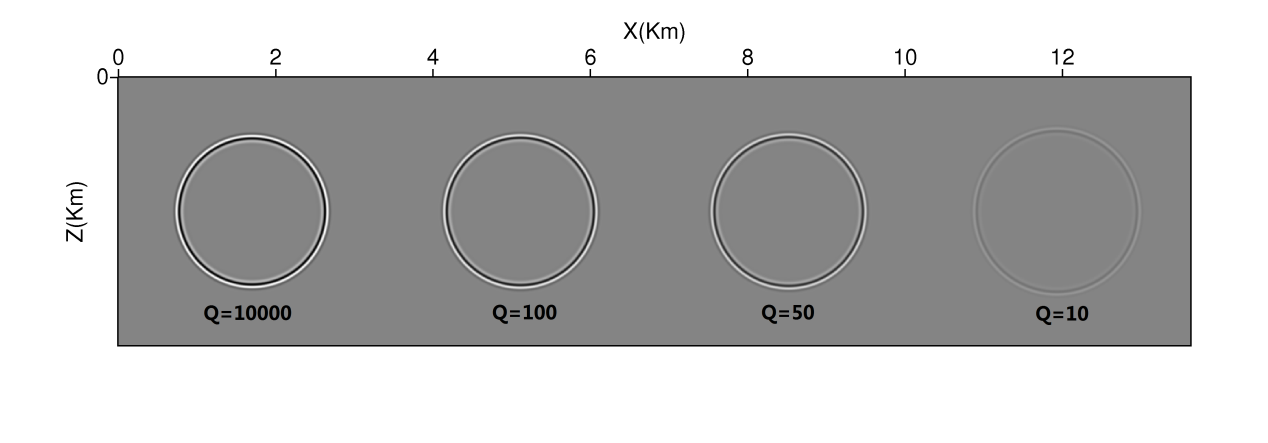
\includegraphics[width=1.0\linewidth]{figure/wave_sls1}
		\fcaption{不同$Q$值在$t=0.35s$的波场快照}{Snapshots of different $Q$  
		models at $t=0.35s$。}[不同$Q$值在$t=0.35s$的波场快照]
		\label{fig:wave_sls1}
\end{figure*}
\begin{figure*}[!htbp]
	    \centering
		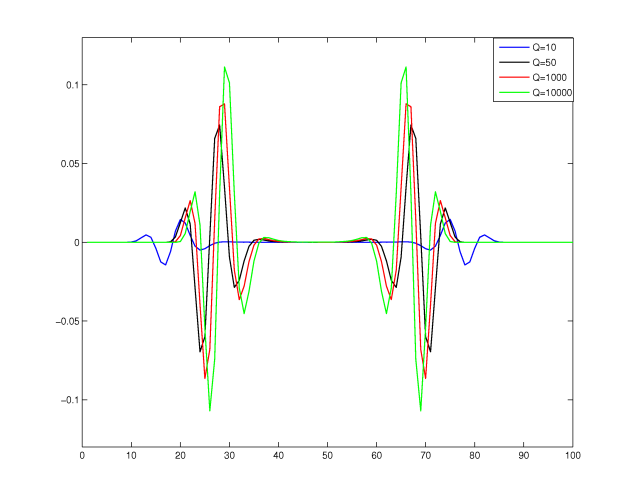
\includegraphics[width=0.5\linewidth]{figure/wave_sls3}
		\fcaption{不同$Q$值在$t=0.35s$,$x=1.7km$处的抽线信息}{The extracted lines  
		of different $Q$ models at $t=0.35s$,$x=1.7km$}[不同$Q$值在$t=0.35s$,$x=1.7km$处的抽线信息]
		\label{fig:wave_sls3}
\end{figure*}
\begin{figure*}[!htbp]
	    \centering
		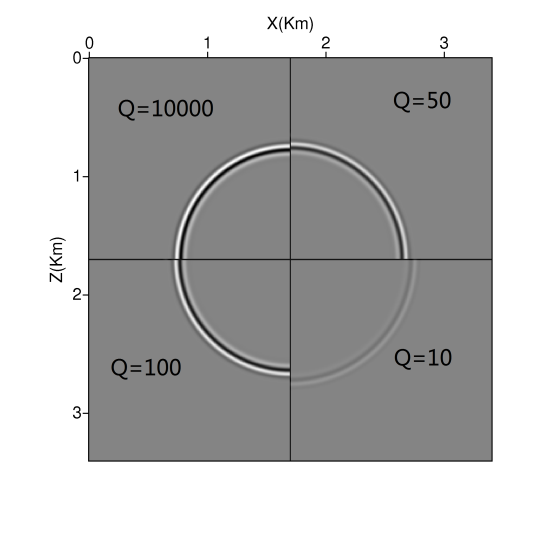
\includegraphics[width=0.5\linewidth]{figure/wave_sls2}
		\fcaption{不同$Q$值在同一时刻波场快照整合图}{Integrated snapshots of different $Q$ 
		model}[不同$Q$值在同一时刻波场快照整合图]
		\label{fig:wave_sls2}
\end{figure*}
\begin{figure*}[!htbp]
	    \centering
		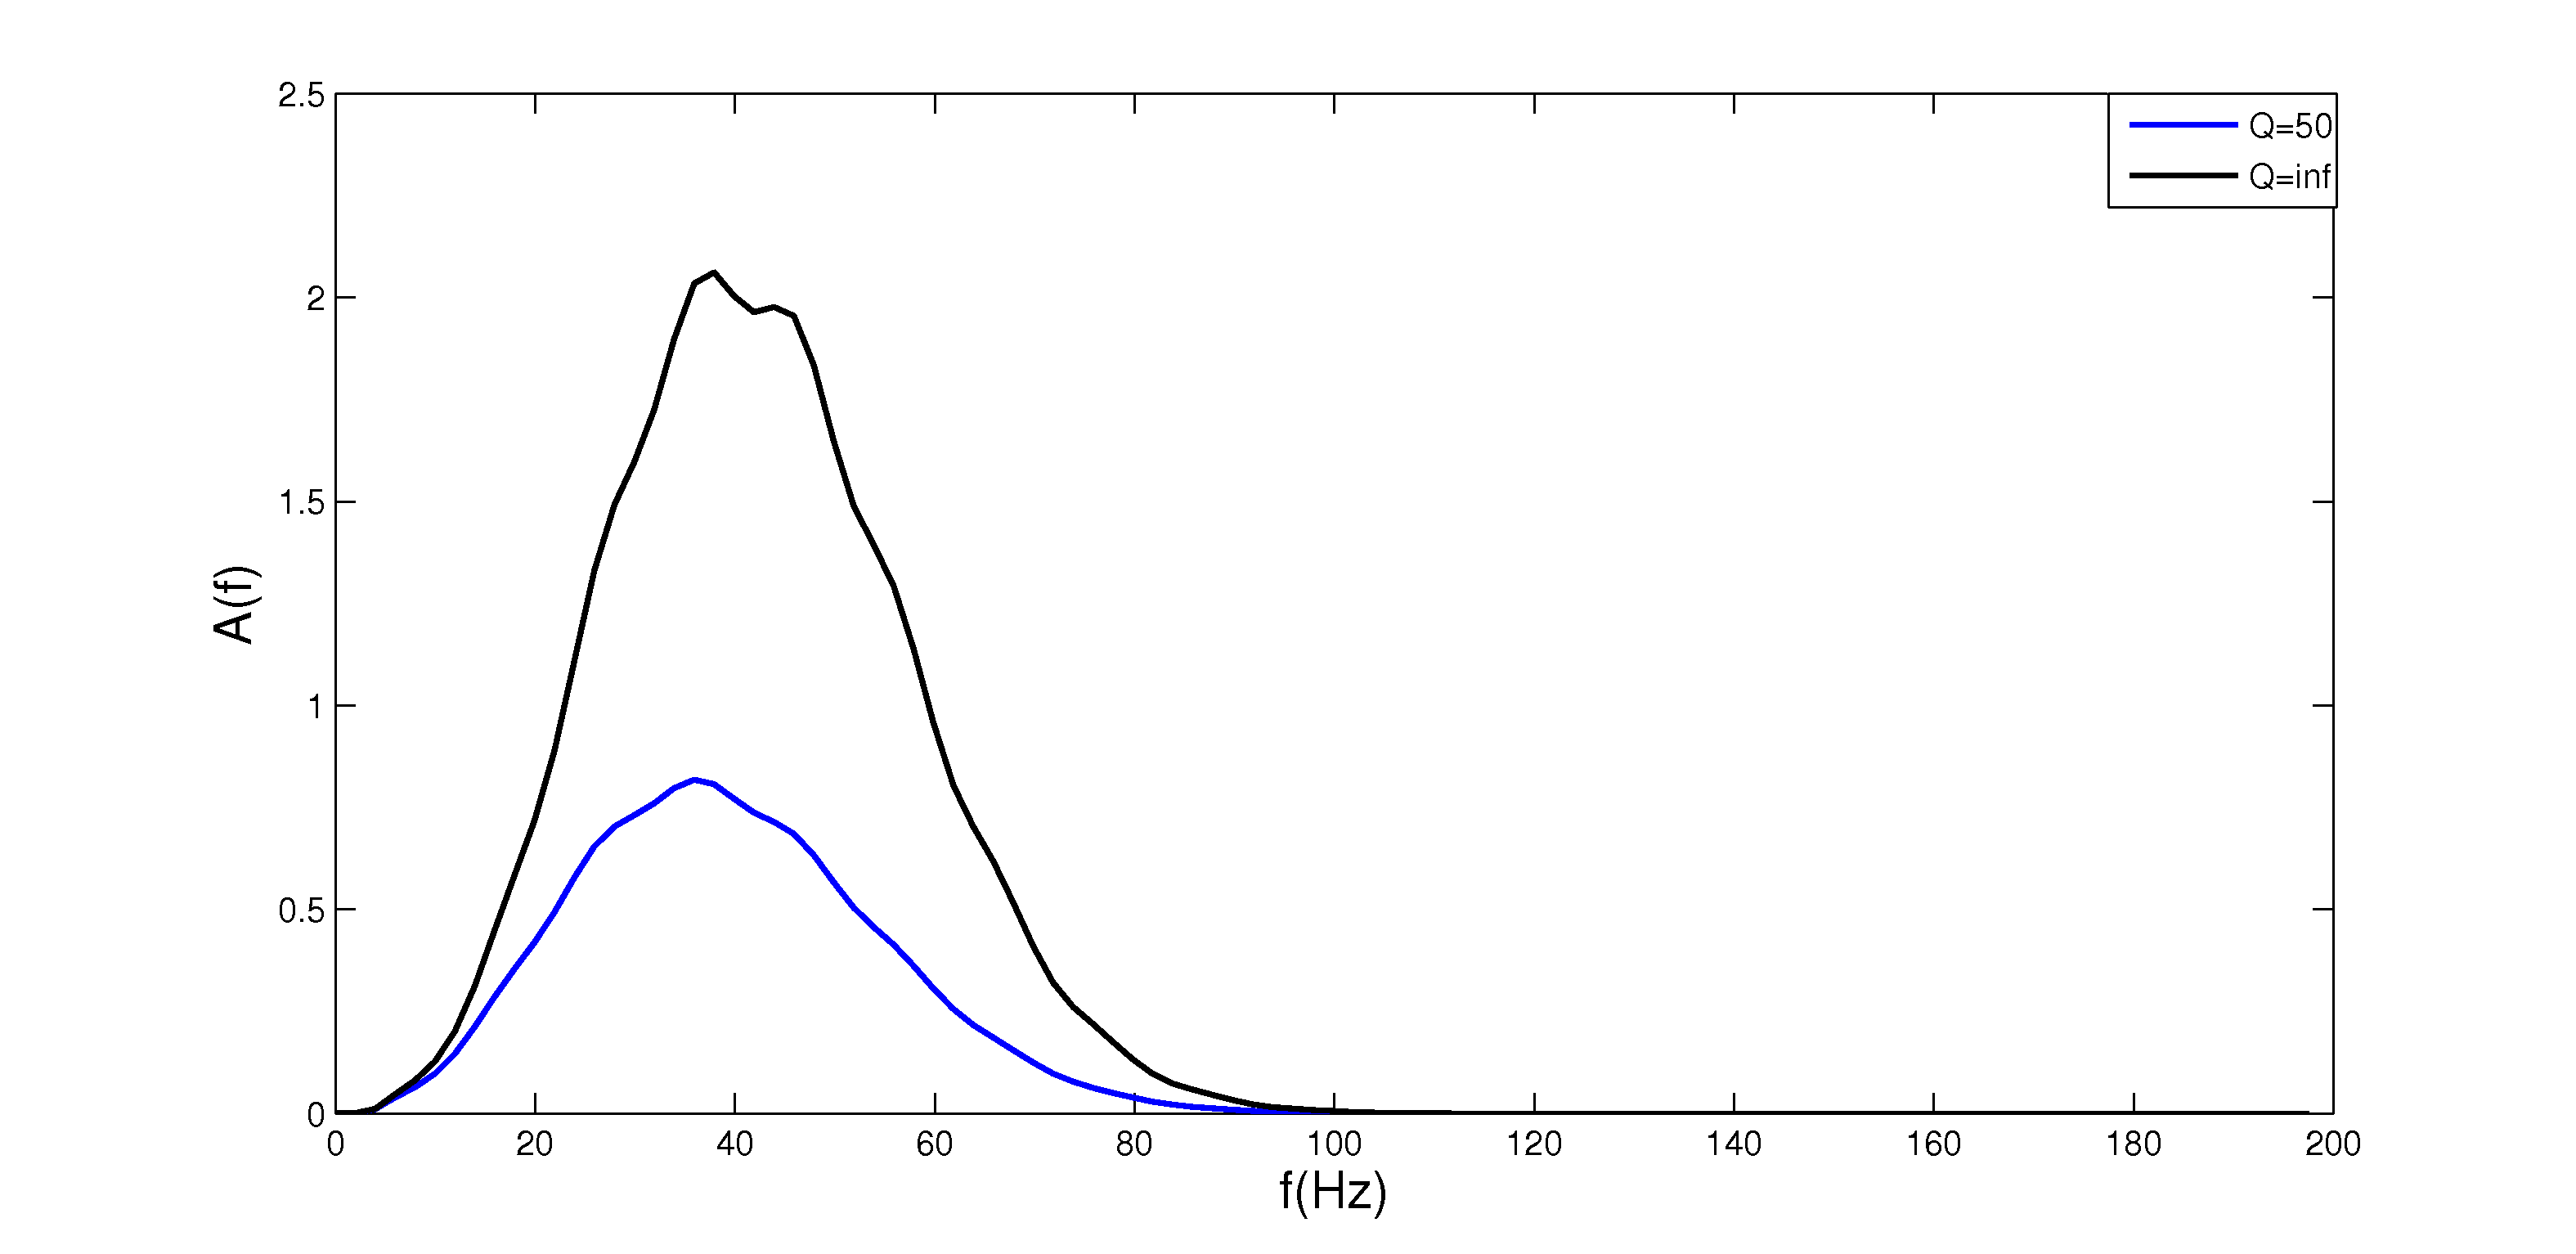
\includegraphics[width=0.7\linewidth]{figure/wave_sls4}
		\fcaption{波场快照抽线的振幅谱}{The amplitude spectrum of extracted lines. 
		}[波场快照抽线的振幅谱]
		\label{fig:wave_sls4}
\end{figure*}
设置一个横向、纵向均为$3.4km$的均匀介质模型,其中纵波速度为$v_p=3km/s$,密度为$\rho=2.0g/cm^3$。
图(\ref{fig:wave_sls1})展示了在$t=0.35s$时刻不同$Q$值的波前快照,图(\ref{fig:wave_sls3})展示
了在$x=1.7km$处的抽线信息,图(\ref{fig:wave_sls2})整合了不同$Q$值的波前快照,图(\ref{fig:wave_sls4})
展示了$Q=50$和声介质波前快照抽线的振幅普。
以上四图从不同的角度证明了粘性介质不仅对地震波振幅有衰减效应而且对相位有较强的改造作用。品质因子的值越小
对地震波的振幅衰减越严重,而且相位有更强的超前效应。从振幅谱可以看出,对高频成分的衰减明显要强于对低频
成分的衰减,这与线性粘弹理论(公式\ref{eq:linear_visco})是一致的。



\vspace{0.5cm}
\subsection{常$Q$模型波动方程模拟}
在勘探地震频段内,认为衰减系数($\alpha\propto 1/Q$)与频率呈近似线性关系,即$Q$在该频段内为常数。
\citeB{kjartansson:1979} 推导出了常$Q$模型的相速度的频散关系:
\begin{equation}
	c=c_0(\frac{\omega}{\omega_0})^\gamma=c_0^2\cos^2(\pi\gamma/2),
\end{equation}
和衰减系数:
\begin{equation}
	\alpha=\tan(\frac{\pi\gamma}{2})\frac{\omega}{v_p}
\end{equation}
式中$c_0$是在给定的参考频率$\omega_0$处的速度。参数$\gamma=1/\pi\tan^{-1}(1/Q)$是一个无量纲的数,对于
任意正$Q$其取值范围为$0<\gamma<0.5$。\citeB{carcione:2002}推导出了常$Q$模型在时间域的粘声波动方程:
\begin{equation}
	\frac{\partial^{2-2\gamma}p}{\partial t^{2-2\gamma}}=c^2\omega_0^{-2\gamma}\bigtriangledown^2p,
	\label{eq:frac}
\end{equation}
式中$\bigtriangledown^2$是拉普拉斯算子,$p(\mathbf{x}t)$是压力波场。方程(\ref{eq:frac})涉及时间的分数
阶偏导数,所以又叫分数阶偏导数方程。在均匀介质中,将波动方程的平面波解
$e^{i(\omega t-\mathbf{k}\cdot\mathbf{x})}$带入方程(\ref{eq:frac})中有如下频散关系:
\begin{equation}
	\frac{\omega^2}{c^2}=(i)^{2\gamma}\omega_0^{-2\gamma}\omega^{2\gamma}\mathbf{k}^2.
	\label{eq:dispersion}
\end{equation}
\citeB{zhu.harris:2014} 从方程(\ref{eq:dispersion})出发,推导了如下近似频散关系:
\begin{equation}
	\frac{\omega^2}{c^2}=-\eta|\mathbf{k}|^{2\gamma+2}-i\omega\tau|\mathbf{k}|^{2\gamma+1}
	\label{eq:dispersion1}
\end{equation}
对应的分数阶常$Q$波动方程为:
\begin{equation}
	\frac{1}{c_0^2}\frac{\partial^2p}{\partial t^2}=\bigtriangledown^2p + \{\eta(-\bigtriangledown^2)^
	{\gamma+1}-\bigtriangledown^2\}p + \tau\frac{\partial}{\partial t}(-\bigtriangledown^2)^{\gamma+
	\frac{1}{2}}p,
	\label{eq:con_equation}
\end{equation}
其中$\eta=-c_0^{2\gamma}\omega_0^{-2\gamma}\cos(\pi\gamma)$,$\tau=-c_0^{2\gamma-1}\omega^{-2\gamma}
\sin(\pi\gamma)$。方程(\ref{eq:con_equation})中的相速度$c_0$和分数阶指数$\gamma$依赖于空间变量
$\mathbf{x}$,通常是非均匀的,这导致用传统方法求解该方程变得非常困难。近年来,低秩近似方法(\citeA{etgen:2009} 
;\citeA{cheng.fomel:2014} )的发展应用使得求解此方程变得容易。用低秩近似求解方程(\ref{eq:con_equation})
的具体实现可参见附录A。另外,\citeB{yao.zhu:2017} 用埃尔米特分布逼近泛函来求解此方程。


方程(\ref{eq:con_equation})右边有三项,第一项为声波项,第二项控制频散,第三项控制衰减。该方程与方程
(\ref{eq:frac})最主要的区别是显示的把衰减项与频散项显示分开,这对地震波逆时偏移成像有重要意义。
图(\ref{fig:wave_frac})展示了均匀介质模型($Q=10,c_0=2164m/s$),不同控制项产生的波前快照。控制衰减项
产生的波场与声波方程产生的波场具有相同的相位,但是其振幅明显较弱;控制频散项产生的波场与声波方程产生的波场
具有相当的振幅,但是其相位有明显的移动。全粘声方程既衰减了地震波的振幅也改造了地震波的相位。
\begin{figure*}[!htbp]
	    \centering
		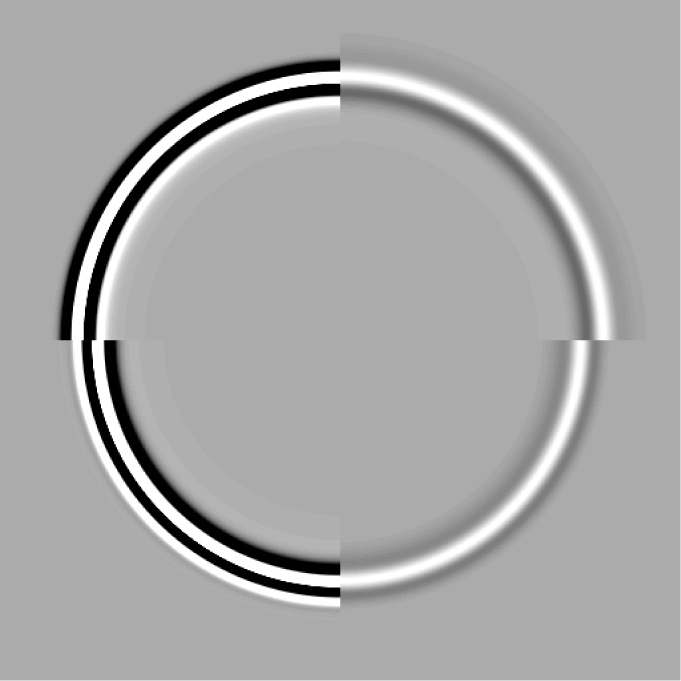
\includegraphics[width=0.5\linewidth]{figure/wave_frac}
		\fcaption{近似常$Q$方程不同控制项产生的波前快照}{Four wavefield parts split by the dashed lines are   
		generated by different formulations。}[近似常$Q$方程不同控制项产生的波前快照]
		\label{fig:wave_frac}
\end{figure*}


\vspace{0.5cm}
\subsection{衰减模型在地震波偏移成像中的应用}
地下介质的强衰减不仅会减弱地震波的振幅,对地震波的相位也有较强的改造。在地震波偏移成像中,如果不考虑衰减
效应会导致在强衰减区成像能量很弱,而且像的位置不聚焦。所以,地震波逆时偏移成像(RTM)中考虑地层衰减效应
特别重要,尤其是在流体饱和的储层和气云区(\citeA{muller.gurevich:2010})。$Q$补偿的成像方法有很多,在数据域
\citeB{hargreaves.calvert:1991}通过反$Q$滤波来补偿地震记录。反$Q$滤波法基于一维假设,不适合复杂情况下的$Q$补偿。
\citeB{fletcher.nichols:2012}匹配源端和检波点端的波场,通过匹配滤波在波的传播过程中补偿衰减效应。滤波器由匹配声波模拟
和粘声模拟结果获得,并在每一步成像之前施加,所以严重依赖于I/O。因为地震衰减是在波的传播过程中发生的,所以通过
修改传播算子在传播过程中补偿$Q$效应是很直接的想法。常用考虑衰减的粘声波动方程有两种,一种是标准线性固体模型,
另一种是常$Q$模型。本节对比这两类方程在$Q$补偿的RTM($Q$-RTM)中的应用。

对于SLS粘声波动方程(\ref{eq:visco}),衰减效应包含于记忆变量中。\citeB{deng.mcmechan:2008}通过改变记忆变量
在方程(\ref{eq:visco})中的正负号来补偿检波点端的振幅损失。这种方法对于弱衰减区域有效,衰减的振幅得以补偿。
但是振幅的衰减和速度的频散都耦合于记忆变量中,通过改变记忆变量符号的方法不能正确校正速度频散效应从而使得在强衰减
区域的成像位置不聚焦。\citeB{bai.chen:2013} 不使用记忆变量而是通过拟微分算子来补偿振幅衰减,忽略相位效应。
以上两种基于SLS粘声波动方程的$Q$-RTM算法均会导致相位变形。

\citeB{zhang.zhang:2010} 用拟微分算子推导出了一种常$Q$粘声方程把振幅衰减和速度频散项区分开来。同样地,
\citeB{zhu.harris:2014}通过频散关系近似,用分数阶拉普拉斯算子推导了另一种常$Q$粘声方程以区分振幅衰减和
速度频散。在$Q$-RTM实现中,这两种分离的常$Q$(DCQ)方程通过改变方程中振幅衰减项(方程\ref{eq:con_equation}右端
第三项)的符号来补偿振幅衰减,而速度频散项(方程\ref{eq:con_equation}右端第二项)保持
不变,从而保证震源端和检波点端波场传播速度相同。在$Q$-RTM中,波场反传是一个能量补偿过程,\citeB{zhang.zhang:2010}
通过在方程中增加一个正则化项来阻止高频噪音的无限放大。而\citeB{zhu.harris1:2014}通过低通Tukey滤波来保持反传
波场的稳定性。

设计一个简单的二维层状模型(图\ref{fig:lens_v})来展示两种方程的$Q$-RTM效果,模型具有五层结构,中间包含两个斜层,
在模型的深部有一个强衰减区(图\ref{fig:lens_q})。用于偏移的合成地震记录是用粘声波方程Born正演产生的,从而去掉
直达波对成像的影响。图(\ref{fig:rtm_no})显示了用声波方程偏移的结果,在强衰减区域的下方,由于没考虑衰减的影响
其成像的能量很弱,并且成像位置轻微偏移正确位置。图(\ref{fig:rtm_sls})是基于SLS方程的$Q$-RTM结果,强衰减区域
下的成像能量得到了补偿,但由于没有正确处理相位的影响,成像不聚焦并且位置偏离正确位置严重。
图(\ref{fig:rtm_con})是基于DCQ方程的$Q$-RTM结果,反传波场能量得到了补偿,因此强衰减区域下方的地层能量得到
了补偿,由于没有改变方程的速度频散关系,正传和反传波场具有相同的速度,所以成像位置是准确的,像的连续性更好。
因此,在存在强衰减的区域,为了得到正确的聚焦的成像结果,$Q$补偿偏移成像是必然选择,并且DCQ方程的偏移结果明显优于
SLS方程。

另外,在粘声最小二乘偏移($Q$-LSRTM)中(\citeA{dutta.schuster:2014};\citeA{sun.fomel:2016}),能量的衰减可以
通过多次迭代来补偿,所以在$Q$-LSRTM中没有必要重新构造传播算子。根据伴随状态法,用伴随方程反传数据残差计算模型的
更新量,无论用SLS方程还是DCQ方程均能得到很好的成像结果。
\begin{figure*}[!htbp]
	    \centering
		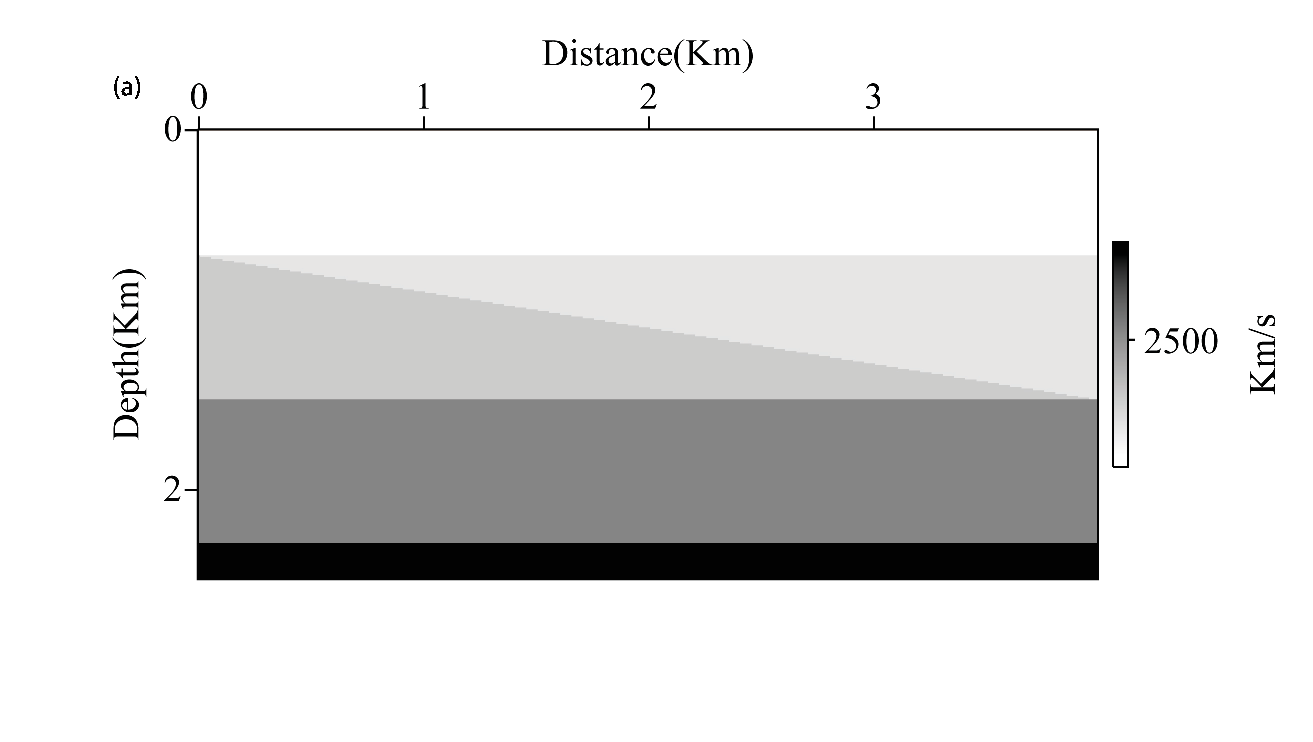
\includegraphics[width=1.0\linewidth]{figure/lens_v.pdf}
		\fcaption{层状速度模型。}{Layered velocity model.   
		}[层状速度模型]
		\label{fig:lens_v}
\end{figure*}
\begin{figure*}[!htbp]
	    \centering
		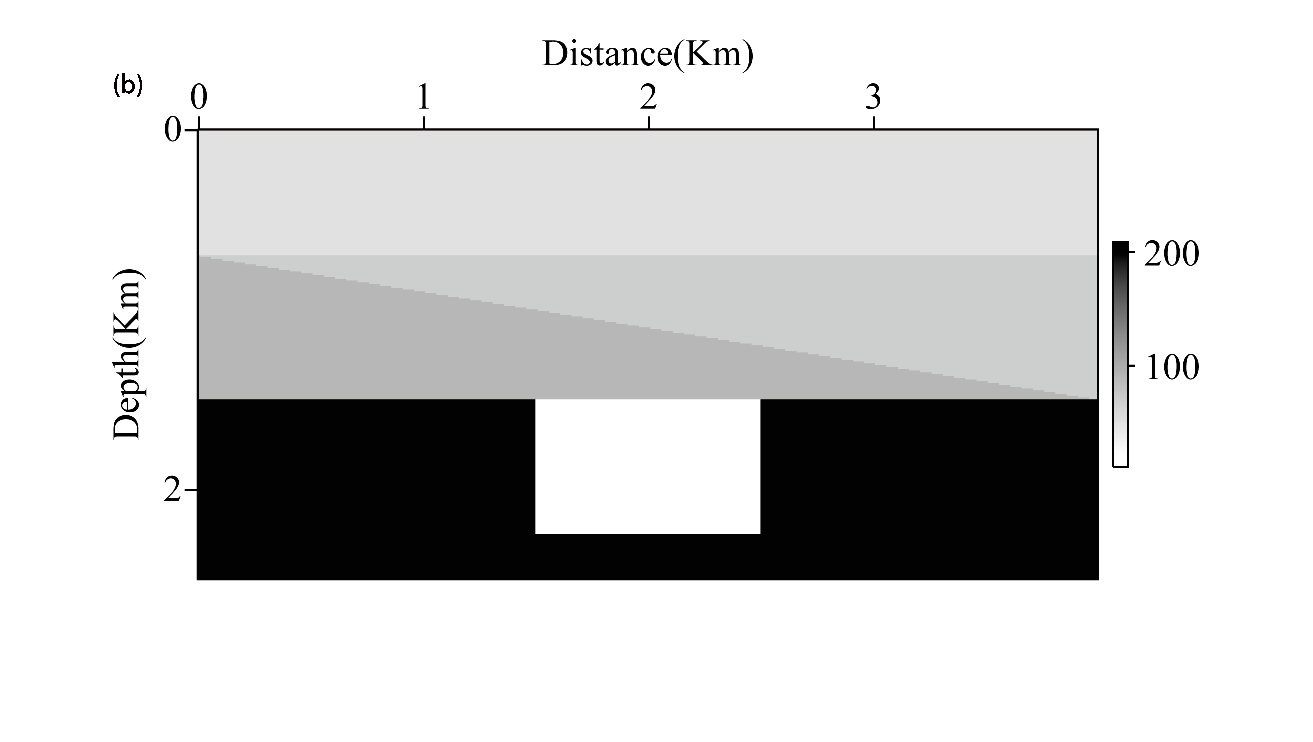
\includegraphics[width=1.0\linewidth]{figure/lens_q.pdf}
		\fcaption{衰减模型。}{Quality factor model.   
		}[衰减模型]
		\label{fig:lens_q}
\end{figure*}
\begin{figure*}[!htbp]
	    \centering
		\includegraphics[width=1.0\linewidth]{figure/rtm_no.pdf}
		\fcaption{不考虑$Q$补偿的RTM结果}{RTM without $Q$-compensation   
		}[不考虑$Q$补偿的RTM结果]
		\label{fig:rtm_no}
\end{figure*}
\begin{figure*}[!htbp]
	    \centering
		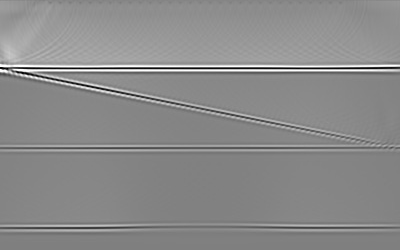
\includegraphics[width=1.0\linewidth]{figure/rtm_sls}
		\fcaption{SLS方程$Q$-RTM结果}{$Q$-RTM using SLS equation   
		}[SLS方程$Q$-RTM结果]
		\label{fig:rtm_sls}
\end{figure*}
\begin{figure*}[!htbp]
	    \centering
		\includegraphics[width=1.0\linewidth]{figure/rtm_con.pdf}
		\fcaption{近似常$Q$方程$Q$-RTM结果}{$Q$-RTM using DCQ equation  
		}[近似常$Q$方程$Q$-RTM结果]
		\label{fig:rtm_con}
\end{figure*}
